\documentclass[tikz]{standalone}
\usepackage[outline]{contour} % glow around text
\usepackage{physics}
\usepackage{xcolor}
\usepackage{etoolbox} %ifthen
\usetikzlibrary{calc}
\usetikzlibrary{arrows,arrows.meta}
\usetikzlibrary{decorations.markings}
\usetikzlibrary{angles,quotes} % for pic (angle labels)
\usetikzlibrary{fadings}
\tikzset{>=latex} % for LaTeX arrow head
\contourlength{1.4pt}

% https://tikz.net/optics_twoslit/

% Colors
\colorlet{wall}{blue!30!black}
\colorlet{myred}{red!70!black}
\colorlet{myblue}{blue!70!black}
\colorlet{myshadow}{blue!30!black!90}
\colorlet{mylightgreen}{green!60!black!70}
% Styles
\tikzstyle{wave}=[myblue,thick]
\tikzstyle{mydashed}=[black!70,dashed,thin]
\tikzstyle{mymeas}=[{Latex[length=3,width=2]}-{Latex[length=3,width=2]},thin]
\tikzstyle{mysmallarr}=[-{Latex[length=3,width=2]}]
% Commands
\newcommand\rightAngle[4]{
  \pgfmathanglebetweenpoints{\pgfpointanchor{#2}{center}}{\pgfpointanchor{#3}{center}}
  \coordinate (tmpRA) at ($(#2)+(\pgfmathresult+45:#4)$);
  \draw[white,line width=0.6] ($(#2)!(tmpRA)!(#1)$) -- (tmpRA) -- ($(#2)!(tmpRA)!(#3)$);
  \draw[mydarkred] ($(#2)!(tmpRA)!(#1)$) -- (tmpRA) -- ($(#2)!(tmpRA)!(#3)$);
}
\newcommand\lineend[2]{
  \def\w{0.1} \def\c{30}
  \draw[mygreen] (#1)++(#2:\w) to[out=#2-180-\c,in=#2+\c] (#1)
                               to[out=#2+\c-180,in=#2-\c]++ (#2-180:\w);
}
\def\tick#1#2{\draw[thick] (#1) ++ (#2:0.1) --++ (#2-180:0.2)}

\begin{document}

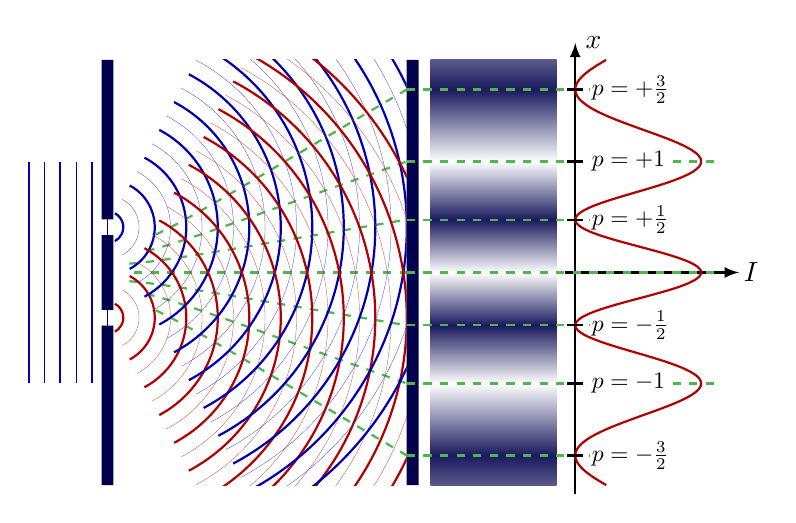
\begin{tikzpicture}[
		nodal/.style={mylightgreen,dashed,thick},
		declare function={
				%xnode(\n,\dn,\lam,\f) = sqrt( (\n^2+(\n+\dn)^2)*\lambd^2/2 - (\n^2-(\n+\dn)^2)^2*\lambd^4/(4*\a^2) - \a^2/4 );
				xnode(\n,\dn,\lam,\f) = \lam/\f*sqrt( \n^2*(\f^2-\dn^2)+\n*\dn*(\f^2-\dn^2)+\dn^2*\f^2/2-(\f^4+\dn^4)/4 );
				ynode(\n,\dn,\lam,\a) = (2*\n*\dn+\dn^2)*\lam/(2*\f);
				intensity(\y,\lam,\a,\Le) = cos(180*\a*\y/(2*\lam*sqrt(\Le*\Le+\y*\y)))^2;
			}
	]

	\def\Le{3.8}       % distance between walls
	\def\H{5.4}       % total wall height
	\def\h{2.8}       % plane wave height
	\def\t{0.15}      % wall thickness
	\def\a{1.15}      % slit distance
	\def\d{0.20}      % slit size
	\def\N{21}        % number of waves
	\def\lambd{0.20}  % wavelength
	\def\R{\N*\lambd} % wave radius
	\def\Nlines{3}    % number of nodal lines
	\def\A{1.6}       % amplitude
	%\def\r{0.06}      % point source radius
	%\def\nmax{10}
	\def\nsamples{100}
	\def\ang{62}

	\begin{scope}
		\clip (-\t/2,-\H/2) rectangle (\Le,\H/2);
		%\clip (-\t/2,0.7*\a) -- (0.6*\Le,\H/2) -- (\Le,\H/2) --
		%      (\Le,-\H/2) -- (0.6*\Le,-\H/2) -- (-\t/2,-0.7*\a) -- cycle;

		% NODAL LINES
		\draw[nodal]
		(0.08*\N*\lambd,0) -- (1.06*\R,0);
		\coordinate (NP0) at (\Le,0);  % to avoid "Dimension too large error"
		\foreach \dn [evaluate={
					\f=\a/\lambd;
					\nmin=2.5+0.2*\dn; %0.501*(-\dn+\f)
					\nmax=10; %(NP0)
					\c=int(\dn<\f);
					\y=\Le/sqrt((\a/(\lambd*\dn))^2-1);
				}] in {1,...,\Nlines}{
				\coordinate (NP+\dn) at (\Le,\y);  % to avoid "Dimension too large error"
				\coordinate (NP-\dn) at (\Le,-\y); % to avoid "Dimension too large error"
				\ifnum\c=1
					\draw[nodal,variable=\n,samples=\nsamples,smooth]
					plot[domain=\nmin:\nmax] ({xnode(\n,\dn,\lambd,\f)},{ynode(\n,\dn,\lambd,\f)})
					-- (NP+\dn);
					\draw[nodal,variable=\n,samples=\nsamples,smooth]
					plot[domain=\nmin:\nmax] ({xnode(\n,\dn,\lambd,\f)},{-ynode(\n,\dn,\lambd,\f)})
					-- (NP-\dn);
				\fi
			}

		% WAVES
		\foreach \i [evaluate={\R=\i*\lambd;}] in {1,...,\N}{
				\ifodd\i
					\draw[myblue,line width=0.8] (0,\a/2)++(\ang:\R) arc (\ang:-\ang:\R);
					\draw[myred,line width=0.8] (0,-\a/2)++(\ang:\R) arc (\ang:-\ang:\R);
				\else
					\draw[myblue!80,line width=0.1] (0,\a/2)++(\ang:\R) arc (\ang:-\ang:\R);
					\draw[myred!80,line width=0.1] (0,-\a/2)++(\ang:\R) arc (\ang:-\ang:\R);
				\fi
			}
	\end{scope}

	% PLANE WAVES
	\foreach \i [evaluate={\x=-\i*\lambd;}] in {0,...,5}{
			\ifodd\i
				\draw[myblue,line width=0.8] (\x,-\h/2) -- (\x,\h/2);
			\else
				\draw[myblue,line width=0.1] (\x,-\h/2) -- (\x,\h/2);
			\fi
		}

	% WALL
	\fill[wall]
	(\t/2,\a/2-\d/2) rectangle (-\t/2,-\a/2+\d/2)
	(\t/2,\a/2+\d/2) rectangle (-\t/2,\H/2)
	(\t/2,-\a/2-\d/2) rectangle (-\t/2,-\H/2)
	(\Le,-\H/2) rectangle (\Le+\t,\H/2);

	% SHADES
	\begin{scope}[shift={(1.08*\Le,0)}]
		\def\yz{\Le/sqrt((\a/\lambd)^2-1)} % m = +- 1/2
		\def\yZ{\Le/sqrt((\a/\lambd/2)^2-1)} % m = +- 1
		\clip (0,-\H/2) rectangle (1.1*\A,\H/2);
		\fill[white] (0,-\H/2) rectangle++ (\A,\H); % to fill seams
		\foreach \i [evaluate={\n=0.5*\i;\yn=\Le/sqrt((\a/(2*\lambd*\n))^2-1);
				}] in {1,...,\Nlines}{
				\ifodd\i % if even
					\fill[myshadow] (0,{-\yn-0.1}) rectangle++ (\A,0.2); % to fill seams
					\fill[myshadow] (0,{ \yn-0.1}) rectangle++ (\A,0.2); % to fill seams
				\fi
			}
		\path[left color=myshadow,right color=myshadow,middle color=white,shading angle={180}]
		(0,{-\yz}) rectangle (\A,{\yz});
		\foreach \i [evaluate={
					\n=0.5*\i;
					\m=0.5*(\i+1);
					\yn=\Le/sqrt((\a/(2*\lambd*\n))^2-1);
					\ym=\Le/sqrt((\a/(2*\lambd*\m))^2-1);
					\dang=mod(\i,2)*180;
				}] in {1,...,\Nlines}{
				\path[left color=myshadow,right color=white,shading angle={\dang}]
				(0,\yn) rectangle (\A,\ym);
				\path[left color=myshadow,right color=white,shading angle={180+\dang}]
				(0,-\yn) rectangle (\A,-\ym);
			}
	\end{scope}

	% INTENSITY
	\begin{scope}[shift={(1.1*\Le+1.1*\A,0)}]
		\draw[->,thick] (-0.08*\A,0) -- (1.3*\A,0) node[right=-2] {$I$}; % I axis
		\draw[->,thick] (0,-0.52*\H) -- (0,0.54*\H) node[right] {$x$}; % x axis
		\draw[nodal] (NP0) --++ (0.15*\Le+2.1*\A,0); % green nodal lines
		\foreach \i [evaluate={\y=\Le/sqrt((\a/(\lambd*\i))^2-1)}] in {1,...,\Nlines}{ % green nodal lines
				\draw[nodal] (NP+\i) --++ ({0.15*\Le+1.1*\A+\A*intensity(\y,\lambd,\a,\Le)},0);
				\draw[nodal] (NP-\i) --++ ({0.15*\Le+1.1*\A+\A*intensity(\y,\lambd,\a,\Le)},0);
			}
		\draw[myred,thick,variable=\y,samples=\nsamples,smooth,domain=-\H/2:\H/2]
		plot({\A*intensity(\y,\lambd,\a,\Le)},\y);
		\foreach \i [evaluate={ % ticks
					\modd=\i; %int(\i);
					\meven=int(\i-1);
					\y=\Le/sqrt((\a/(\lambd*\i))^2-1);
				}] in {1,...,\Nlines}{
				\ifodd\i
					\tick{0,-\y}{180} node[right=0,scale=0.85] {$p=-\frac{\modd}{2}$};
					\tick{0,\y}{180} node[right=0,scale=0.85] {$p=+\frac{\modd}{2}$};
				\else
					\tick{0,-\y}{180} node[right=0,scale=0.85, fill=white] {$p=-\meven$};
					\tick{0,\y}{180} node[right=0,scale=0.85, fill=white] {$p=+\meven$};
				\fi
			}
	\end{scope}

\end{tikzpicture}
\end{document}
